\newcommand{\degree}{\ensuremath{^{\circ}}}

\chapter{Kreslenie molekuly}

Po tom čo získame a aplikujeme mapovanie medzi šablonovou a cieľovou molekulou RNA,
získame cieľovú molekulu s čiastočnou vizualizáciou, ktorej zvyšok potrebujeme dopočitať.

Príklad ako to vyzerá je na obrázku \ref{obr:frog_to_human}, kde sme
namapovali sekundárnu štruktúru malej podjednotky rRNA 23S žaby (X04025) do
obrázka sekundárnej štruktúry malej podjednotky rRNA 23S človeka.
Ako si môžeme všimnúť, v obrázku (najmä v spodnej časti) sú bázy nakreslené
sivo - tie sa chystáme zmazať. V obrázku nám tak vzniknú prázdne miesta.
Naopak po insertoch potrebujeme vypočítať, kam umiestníme daný pár,
resp. samotnú bázu, prípadne pre ňu musíme urobiť miesto a posunúť zvyšok
molekuly. Update vrcholu nerobí žiadne štruktúrne zmeny, zmení sa iba
báza na danom mieste.

\begin{figure}
  \centering
  %trim=left bottom right top
  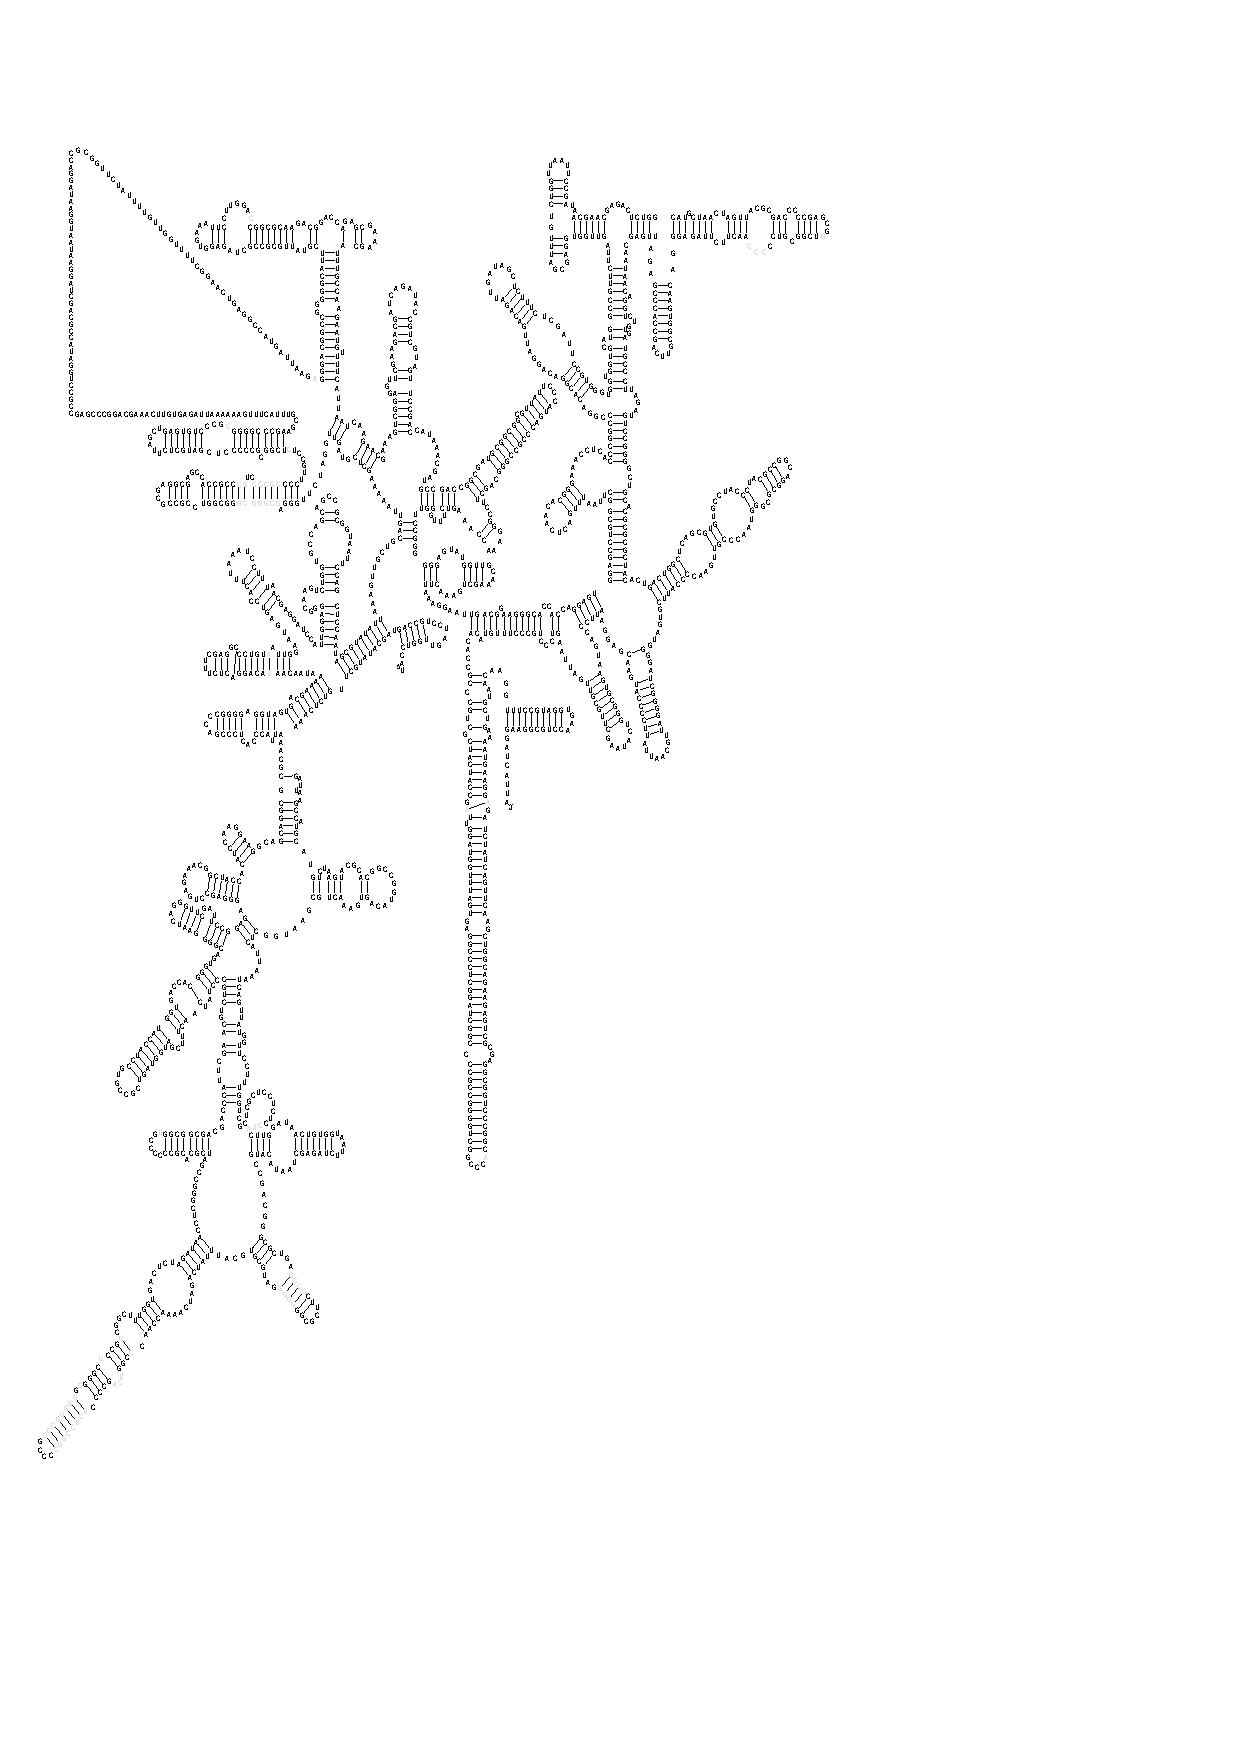
\includegraphics[clip, trim=0 5cm 6cm 2cm, width=1\textwidth]{../img/african_frog-to-human-mapped}
  \caption{Namapovanie rRNA žaby do obrázka rRNA človeka z \ref{obr:human_crw}, sivou sú označené mazané bázy}
  \label{obr:frog_to_human}
\end{figure}

Čiastočnej vizualizácie sa chceme dotýkať čo najmenej. To znamená, že všetky zásahy sa
snažíme robiť iba v miestach, ktoré sa zmenili - boli dotknuté vkladaním alebo mazaním báz.

Jediné dve výnimky budú normalizácia vzdialeností medzi bázovými pármi a vyrovnávanie stemov.





\section{Normalizácia vzdialeností v bázových pároch a vyrovnavanie stemov}

Tieto dve výnimky sme sa rozhodli urobiť, keďže časté výnimky nám sťažovali
prácu a veci, ktoré predpokladáme, že v obrázku nájdeme neboli vždy skutočnosťou.

Ako príklad môžeme uviesť, že ak chceme nakresliť nový bázový pár a máme nakreslený
rodičovský párový vrchol. Následne v smere od jeho rodiča (nášho prapredka) kreslíme nový
bázový pár. Tu môže nastať chyba, ktorú ilustrujeme na obrázku \ref{obr:insert_stem_error}.

\begin{figure}[H]
  \centering
  %trim=left bottom right top
  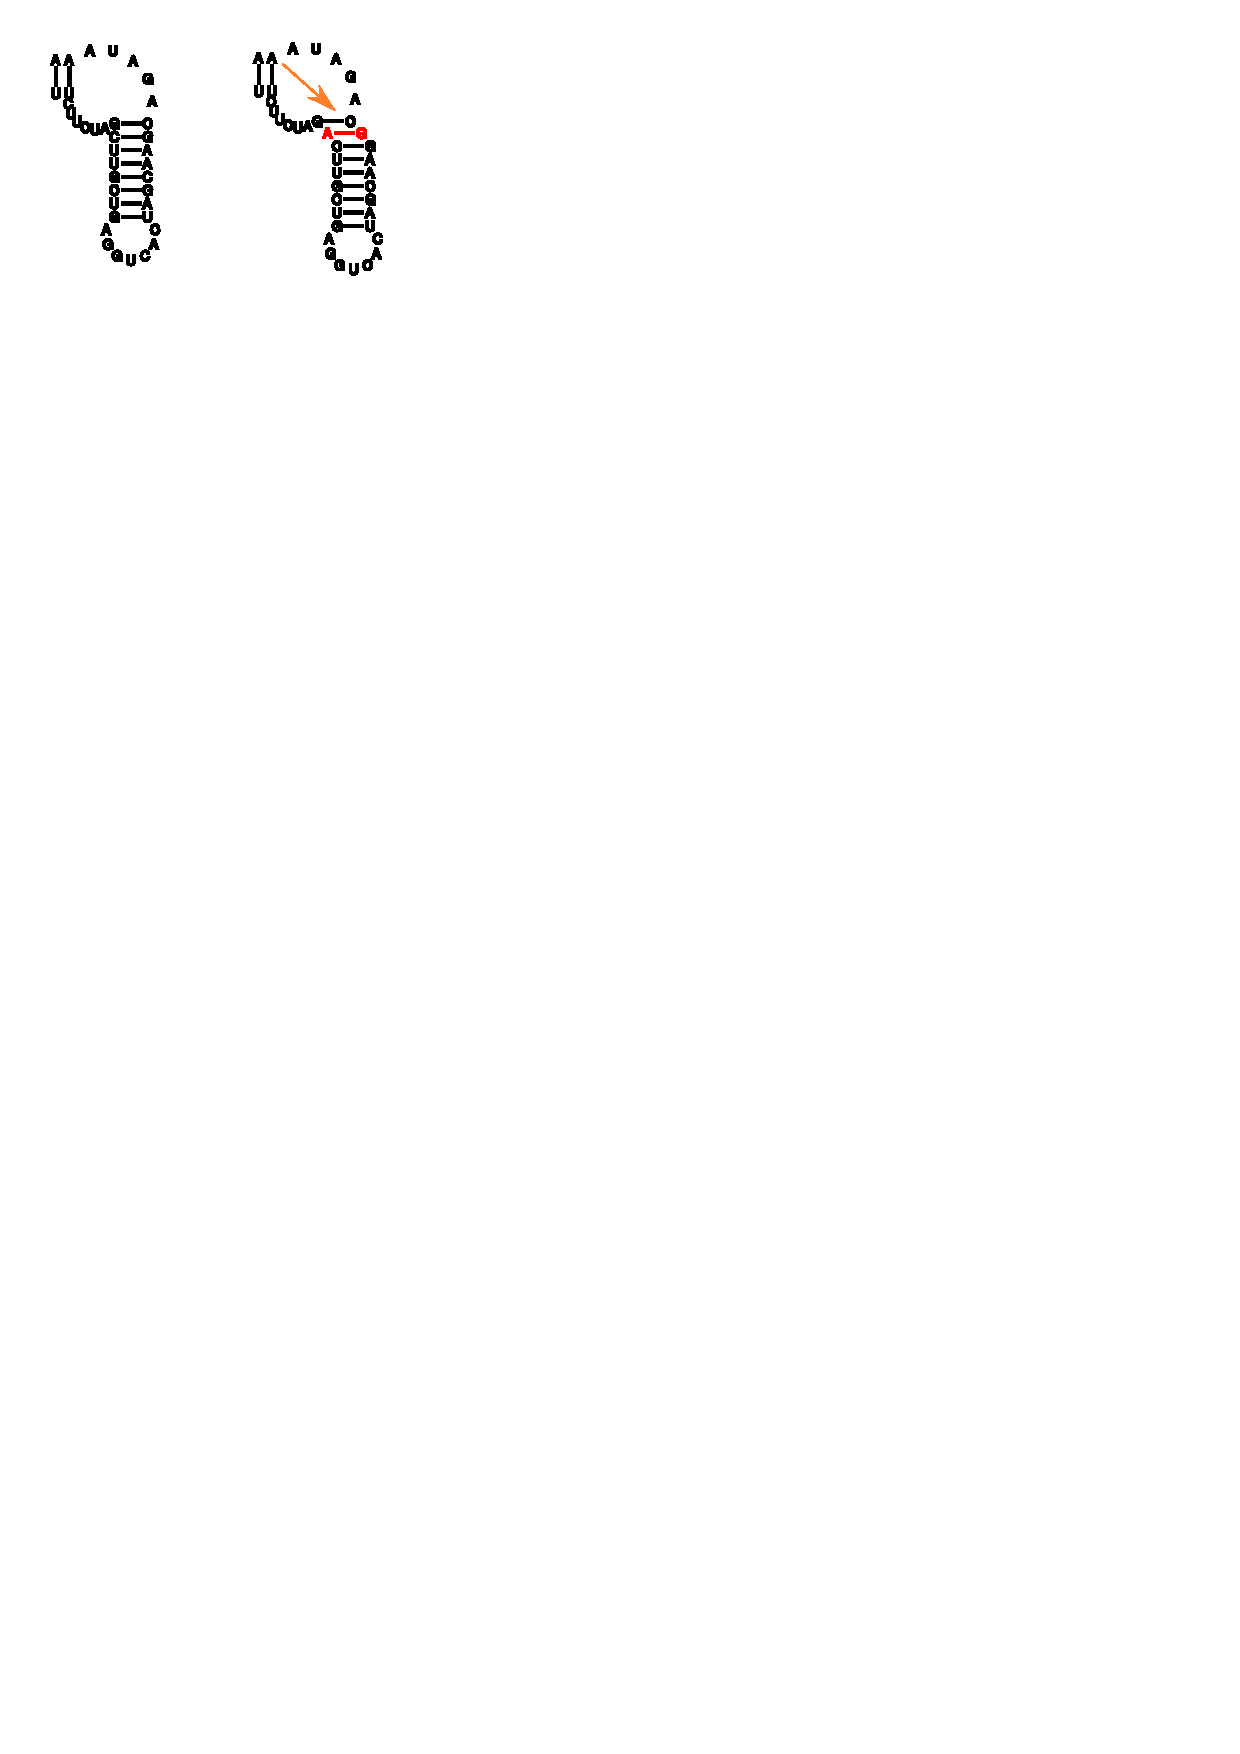
\includegraphics[clip, trim=0 24.5cm 14cm 0]{../img/alg/even_stem/error_insert}
  \caption{Možná chyba pri vkladaní nového bázového páru}
  \label{obr:insert_stem_error}
\end{figure}

Vyrovnávací algoritmus prejde všetky stemy a z ich začiatkov vedie priamku na ktorej
majú podľa pravidla byť uložené všetky stemové vrcholy. Následnými rotáciami
a posunutiami podstromov ich uložíme na miesto.




\section{Operácie na stromoch}

Čitateľa zoznámime s 2 operáciami, ktoré budeme vykonávať na molekule. Tie využijeme
ako pri vkladaní, tak aj pri mazaní vrcholov zo stromu.

\newcommand{\degree}{\ensuremath{^{\circ}}}

\chapter{Kreslenie molekuly}

Po tom čo získame a aplikujeme mapovanie medzi šablonovou a cieľovou molekulou RNA,
ziskame cieľovú molekulu s čiastočnou vizualizáciou, ktorej zvyšok treba dopočitať.

Po operáciach delete ostávajú v molekule prázdne diery, naopak po insertoch potrebujeme
vypočítať, kam umiestnime bázový pár, resp. samotnú bázu, prípadne ešte potrebujeme pre
ňu urobiť miesto. Update vrcholu v strome nerobí žiadne štruktúrne zmeny, zmení sa iba
názov bázy na danom mieste.

Sekundárna štruktúra RNA obsahuje množstvo motivov popisaných na obrázku \ref{obr:RNA_motifs}.
Vo všeobecnosti ale sa každý z týchto motivov skladá zo stemu a loopu.

Stemom budeme ďalej nazývať časť RNA, ktorá zodpovedá vnútornému vrcholu v strome. Loop
budeme označovať listy v RNA strome (lese), nezáleží či je to bulge, interior loop, hairpin
alebo multibranch loop, ako aj ukazuje obrázok \ref{obr:RNA_motifs_stem_loop}.

Stem začína vždy v najvyššom vrchole stromu (v smere ku koreňu), ktorý je zároveň vnútorným
vrcholom a nemá žiadnych súrodencov, ktorý by boli rovnako vnútornými vrcholmi.
To znamená, že do multibranch loop vchádza 1 stem (ten tu konci) a vychádza z nej niekoľko nových stemov.
Naopak pre bulge a interior loop jeden stem vchádza do štruktúry ale pokračuje ďalej.

\begin{figure}[H]
\centering
\fbox{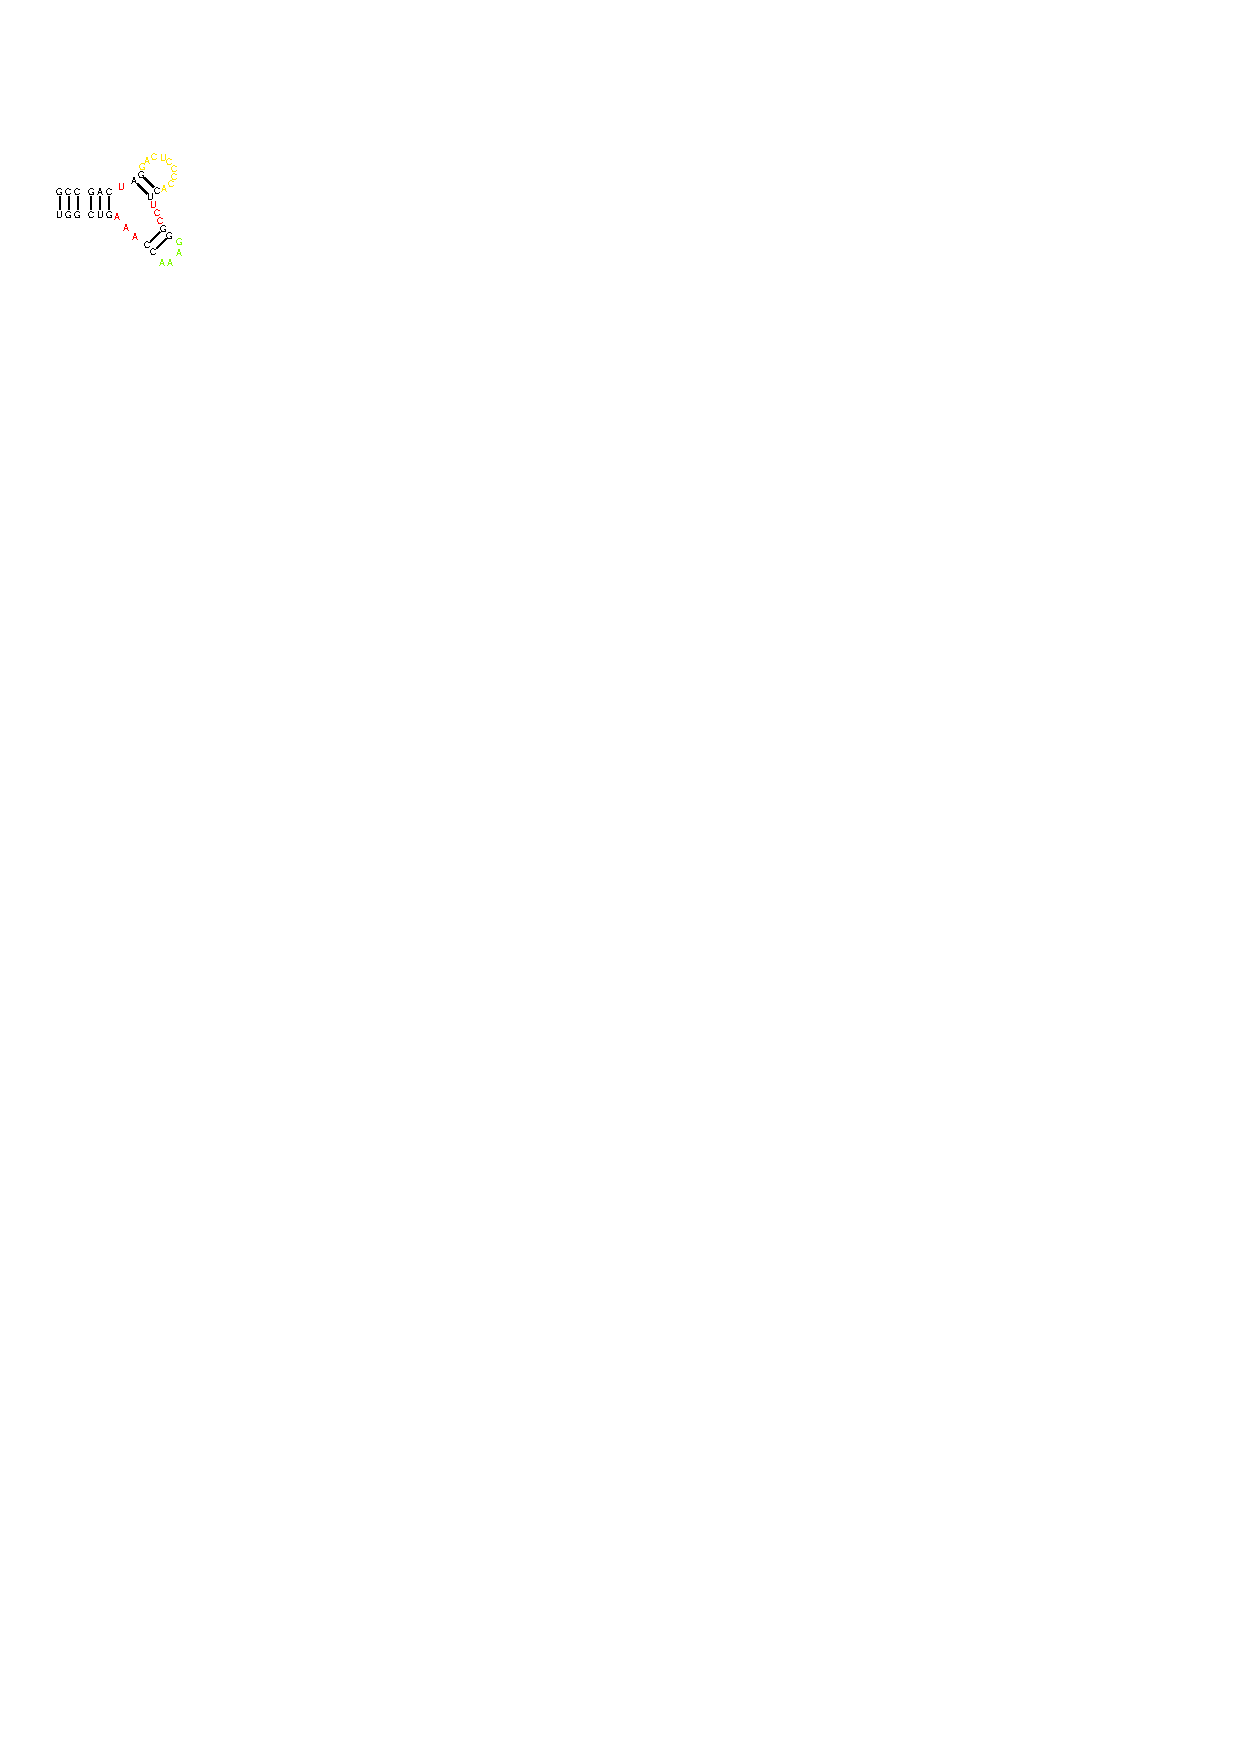
\includegraphics[trim=0.3cm 24.7cm 17cm 2cm]{../img/stem_loop-colored}}
\caption{Rozlisenie stemov a loopov v molekule: cierne su stemy, farebne odlisene su bazy patriace do jednej loopy}
\label{obr:RNA_motifs_stem_loop}
\end{figure}

\section{Štruktúry v RNA}

V článku od \citet{RNA_DRAW} autori popisujú pravidlá vizualizácie sekundárnej štruktúry RNA.

Nakreslenie musí byť rovinné bez krížení, bázy tvoriace rôzne druhy loopov musia ležať na kružniciach
a bázy tvoriace stem majú ležať na priamke.
Ďalším pravidlom je, že vzdialenosť medzi bázami má byť konštantná, či už vzdialenosť medzi bázami jedného páru,
alebo bázami sekvencie.

Ako je ukázane na obrázku \ref{obr:RNA_full}, pravidla niesu niekedy rešpektované. To zťažuje pouzitie obrazka
ako šablony, kedže vo výslednom obrázku chceme všetky tieto pravidlá rešpektovať.

\section{Algoritmus}
Čiastočnej vizualizácie, ktorú dostávame z mapovania sa chceme dotýkať čo najmenej. To znamená,
že všetky zásahy sa snažíme robiť iba v miestach, ktoré boli dotknuté vkladaním alebo mazaním báz.

Jediné výnimky sú normalizácia vzdialensti medzi bázovými pármi a vyrovnávanie stemov.

\subsection{Normalizácia vzdialeností v bázových pároch a vyrovnavanie stemov}

Ako bolo uvedené, stemom rozumieme nevetviacu sa časť stromu tvorenú iba bázovými pármi.

Algoritmus normalizácie vzdialeností medzi vrcholmi bázových párov stojí iba v preiterovaní celého stromu
a ak nejaké párové vrcholy sú od seba príliž vzdialené, priblíži ich k sebe.

Vyrovnávací algoritmus prechádza všetky stemy. Z ich začiatkov vedie priamku, na ktorej majú byť podľa pravidla uložené
všetky stemove vrcholy. Rotáciami a posunutiami podstromov vieme docieliť to, aby vrcholy stemu na tejto priamke ležali.

% TODO obrázok vyrovnávania

\subsection{Operácie na stromoch}

Čitateľa zoznámime s 2 operáciami, ktoré budeme vykonávať na molekule. Tie budeme používať nezávisle
na tom, či vrcholy do stromu vkladáme alebo mažeme.

\begin{algorithm}
  \caption{Rozloženie báz na kružnicu}
  \label{alg:operácia_circle_reinsert}
  \begin{algorithmic}[1]
    \Procedure {rozlozBazy}{Begin, End, Bases}
      \State $n \gets$ veľkosť zoznamu báz $Bases$
      \State $\Gamma \gets$ dostatočne veľká kružnica pre $n$ bodov prechádzajúca bodmi $Begin$ a $End$
      \State $\Pi \gets$ rozdel kruhový obluk kružnice $\Gamma$ od $Begin$ po $End$ na $n$ bodov
      \ForAll{$i$ in 1 .. $n$}
        \State nastav pozíciu bázy $Bases[i]$ na bod $\Pi[i]$
      \EndFor
    \EndProcedure
  \end{algorithmic}
\end{algorithm}

\begin{algorithm}
  \caption{Posunutie podstromu}
  \label{alg:operacia_tree_shift}
  \begin{algorithmic}[1]
    \Procedure {posunPodstrom}{Root, Vector}
      \ForAll {vrchol $V$ v podstrome vrcholu $Root$}
        \If {vrchol $V$ už má určenu pozíciu, t.j. nieje práve vložený}
          \State pripočítaj k pozicií bázy $V$ vektor $Vector$
        \EndIf
      \EndFor
    \EndProcedure
  \end{algorithmic}
\end{algorithm}

Ako sme písali už skôr, všetky loop štruktúry majú byť uložené na kružniciach. K tomu nám pomôže funkcia
\ref{alg:operacia_circle_reinsert}. Tá dostáva na vstupe zoznam báz $Bases$ a dva body v rovine, $Begin$ a $End$.
Týmito bodmi potrebujeme viesť kružnicu, ktorá bude dostatočne veľká, teda aby na ňu všetky bázy zo zoznamu vošli.
Veľkosťou kružnice v tomto prípade myslíme dĺžku kruhového obluku medzi vrcholmi $Begin$ a $End$.

V našom programe používame iteračný algoritmus, ktorý ju pomaly zväčšuje alebo zmenšuje.
Nakoniec buď nájde kružnicu, ktorej veľkosť je optimálna, alebo ani na maximálny počet krokov takú kružnicu nenájde
a tak vráti tu z posledného kroku. Na obrázku \ref{obr:insert_circle_hairpin} vidíme celý algoritmus zväčšovania kružnice.

\begin{figure}
  \begin{subfigure}{0.3\textwidth}
    \fbox{\includegraphics[trim=1cm 24.5cm 17cm 2.5cm]{../img/alg-insert/circle-small}}
  \end{subfigure}
  \begin{subfigure}{0.3\textwidth}
    \fbox{
\includegraphics[trim=1cm 24.5cm 17cm 2.5cm]{../img/alg-insert/circle-big}}
  \end{subfigure}
  \begin{subfigure}{0.3\textwidth}
    \fbox{\includegraphics[trim=1cm 24.5cm 17cm 2.5cm]{../img/alg-insert/alg-insert/circle-big-end}}
  \end{subfigure}

  \caption{Priklad zvacsovania kruznice a insertu do hairpinu}
  \label{obr:insert_circle_hairpin}
\end{figure}

Operácia v rámci algoritmu \ref{alg:operacia_tree_shift} nám pomôže urobiť miesto na novo vložené bázové páry,
alebo naopak ak sme niečo zmazali, tak dokáže celý podstrom pritiahnuť späť.

\subsection{Vkladanie nového vrcholu do stromu}

Pri vkladaní nového vrcholu do stromu môžu nastať nasledovné možnosti.

Ak vkladáme list do hairpinu, je to jednodúche, potrebujeme iba použiť procedúru z algoritmu \ref{alg:operacia_circle_reinsert}
s parametrami $Begin = $ požicia prvej bázy z bázového páru, $End = $ požičia druhej bázy z páru
a $Bases = $ zoznam všetkých potomkov.

Trochu zložitejšie je to pri vkladaní listu do stemu. V tomto prípade buď už stem obsahoval nejaký loop, alebo vzniká nová.
Najprv potrebujeme upraviť vzdialenosť medzi vrcholmi stemu, teda posunuť celý podstrom aby nám dané bázy vošli.
To vyriešime algoritmom \ref{alg:operacia_tree_shift}. Následne nájdeme kružnicu a bázy na ňu naukladáme.

Vkladanie bázového páru do stemu je jednoduché. Najprv posunieme celý podstrom a urobíme tak miesto pre novú dvojicu
báz, a potom ich uložíme na pozíciu kde by mala patriť. Môže sa stať, že vložením vrcholu do stemu zdedíme niekoľko
listov z predka. V tomto prípade iba použijeme operáciu vloženia vrcholu a updatu loopov pred aj za vloženým vrcholom.

\subsection{Modifikácia multibrach loop}

Modifikácia multibranch loop je zložitejšia ako všetky predchádzajúce prípady. Obrázky sú väčšinou ručné upravené tak,
aby bol čo najkompaktnejší a kvôli tomu sa často nerešpektujú pravidlá o kružnicovom tvare štruktúry.
Kvôli tomu sa snažíme do tejto štruktúry nezasahovať, ak sa to dá.

Prekresleniu celej štruktúry sa môžeme vyhnúť napríklad pri zmene počtu listov medzi jednotlivými vetvami.
Ak je zmena dostatočne malá, môžeme vrcholy roztiahnuť, alebo naopak priblížiť k sebe.

Ak sa jedná o pridanie/odobratie celej vetvy stromu, modifikácií sa nevyhneme. V tom prípade potrebujeme
rozdistribuovať všetky vrcholy patriace do loop na kružnicu. Je to podobný proces ako sa používa iba pre samotné loopy,
ale potrebujeme posúvať celé podstromy a zrotovať ich správnym smerom.

\subsection{Mazanie vrcholu zo stromu}

Mazanie považujeme za inverznú operáciu voči vkladaniu do stromu. Vzhľadom k tomu, používame rovnaké operácie
rozdistribuovania vrcholov v loope, alebo posúvanie podstromu, ktoré sa deje v tomto prípade opačným smerom
k predkovi.



Ako sme písali už skôr, všetky loop štruktúry majú byť uložené na kružniciach.
K tomu nám pomôže funkcia \ref{alg:operacia_circle_reinsert}.
Tá dostáva na vstupe zoznam báz $Bases$ a dva body v rovine, $Begin$ a $End$.
Týmito bodmi potrebujeme viesť kružnicu, ktorá bude dostatočne veľká, aby
na ňu všetky bázy zo zoznamu vošli. Veľkosťou kružnice v tomto prípade myslíme
dĺžku jej kruhového oblúku medzi vrcholmi $Begin$ a $End$.

V našom programe používame iteračný algoritmus. Ten začne s kružnicou so stredom
medzi $Begin$ a $End$ bodmi a pomaly ju zväčšuje alebo zmenšuje.
Nakoniec buď nájde kružnicu, ktorej veľkosť je optimálna, alebo ani na maximálny
počet krokov takú kružnicu nenájde a tak vráti tú z posledného kroku.
To sa môže stať napríklad, ak je samotná vzdialenosť medzi bodmi príliš veľká.

Na obrázku \ref{obr:insert_circle_hairpin} vidíme celý algoritmus zväčšovania kružnice.
Začíname kružnicou medzi $Begin$ a $Eend$ bodmi, ktoré reprezentujú bázy posledného
páru v smere $5' \to 3'$. V ďalších dvoch iteráciách zväčšujeme kružnicu až kým
nieje dostatočne veľká pre daný počet báz. Následne vrcholy hairpinu
na ňu uložíme.
Pôvodné vrcholy sú označené modrou, vložené sú zase červené I.

\renewcommand{\wi}{0.24\textwidth}

\begin{figure}
  \begin{subfigure}{\wi}
%trim=left bottom right top
    
\includegraphics[trim=1cm 24.5cm 17.5cm 2.5cm]{../img/alg/insert/1/circle-small-begin}
  \end{subfigure}
  \begin{subfigure}{\wi}
    \includegraphics[trim=1cm 24.5cm 17.5cm 2.5cm]{../img/alg/insert/1/circle-small}
  \end{subfigure}
  \begin{subfigure}{\wi}
    
\includegraphics[trim=1cm 24.5cm 17.5cm 2.5cm]{../img/alg/insert/1/circle-big}
  \end{subfigure}
  \begin{subfigure}{\wi}
    \includegraphics[trim=1cm 24.5cm 17.5cm 2.5cm]{../img/alg/insert/1/circle-big-end}
  \end{subfigure}

  \caption{Príklad zväčšovania kružnice a následné vloženie báz}
  \label{obr:insert_circle_hairpin}
\end{figure}





\subsection{Vkladanie nového vrcholu do stromu}

Pri vkladaní nového vrcholu do stromu môžu nastať nasledovné možnosti.

Ak vkladáme listy do hairpinu, je to jednoduché. Potrebujeme iba použiť
procedúru z algoritmu \ref{alg:operacia_circle_reinsert}
s parametrami $Begin = $ požicia prvej bázy z bázového páru, $End = $ pozícia
druhej bázy z páru a $Bases = $ zoznam všetkých potomkov.
Príklad sme už ukázali na obrázku \ref{obr:insert_circle_hairpin}.

Trochu zložitejšie je to pri vkladaní listu do stemu. V tomto prípade buď už stem
obsahoval nejaký loop, alebo musíme vytvoriť novú. Potrebujeme upraviť vzdialenosť
medzi vrcholmi stemu, teda posunuť celý podstrom tak, aby nám tu všetky bázy vošli.
To vyriešime algoritmom \ref{alg:operacia_tree_shift}. Následne postupujeme
rovnako ako pri vkladaní nukleotidu do hairpinu - nájdeme kružnicu a bázy
na ňu naukladáme.

Vloženie bázového páru do stemu je jednoduché. Najprv posunieme celý podstrom
a tým urobíme miesto pre novú dvojicu báz. Následne ich uložíme na pozíciu kam patria.
Názorný príklad vkladania je na obrázku \ref{obr:insert_stem}.
Môže sa stať, že zdedíme niekoľko nepárových báz z predka. V tom prípade iba
znovu prekreslíme tieto loopy.


\renewcommand{\wi}{0.45\textwidth}

\begin{figure}
  \centering
  \begin{subfigure}{\wi}
%trim=left bottom right top
    \includegraphics[clip, trim=1cm 25cm 14cm 1cm, width=1\textwidth]{../img/alg/insert/stem}
    \caption{Vkladanie bázových párov}
  \end{subfigure}
  \begin{subfigure}{\wi}
%trim=left bottom right top
    \includegraphics[clip, trim=8cm 25cm 7cm 1cm, width=1\textwidth]{../img/alg/insert/stem}
    \caption{Vytvorenie novej loopy v steme}
  \end{subfigure}
  \caption{Vkladanie báz do stemu}
  \label{obr:insert_stem}
\end{figure}




\subsection{Modifikácia multibrach loop}

Modifikácia multibranch loop je zložitejšia ako všetky predchádzajúce prípady.
Obrázky sú väčšinou ručné upravené tak, aby bol čo najkompaktnejší a kvôli tomu
sa často nerešpektujú všetky pravidlá, napríklad kružnicový tvar štruktúry.

Kvôli tomu sa snažíme do tejto štruktúry nezasahovať, ak je to možné.
Vyhnúť sa tomu môžeme napríklad pri malej zmene počtu listov medzi jednotlivými vetvami.
Ak je dostatočne malá, môžeme sa pokúsiť vrcholy roztiahnúť od seba, alebo naopak ich
priblížiť k sebe a tak viac využiť miesto medzi vetvami.

Naopak, ak sa jedná o pridanie, alebo odobratie celej vetvy, modifikácií sa nevyhneme.
V tom prípade rozdistribuujeme vrcholy z loopy (spolu so spárovanými bázami tvoriacimi
vetvy) na kružnicu. Je to podobný proces, ako používame iba pre samotné loopy,
ale potrebujeme naviac vetvy zrotovať do správneho smeru.

Obidva tieto prípady sú znázornené na obrázku \ref{obr:insert_multibranch}
\footnote{Význam použitých farieb v obrázkoch popisuje tabuľka \ref{tab:color_coding}.
  Zatiaľ nám stačí červená - to sú vkladané nukleotidy.},
v obidvoch častiach vizualizujeme sekundárnu štruktúru rRNA človeka z obrázka \ref{obr:human_crw}.
V prvej časti sme sa prekresľovaniu celej štruktúry vyhli a nukleotidy sme
priblížili k sebe. V druhej sme už vkladali celú vetvu stromu a tak sme museli
celú štruktúru prekresliť. Spoločné podčasti sú označené číslami a šípka označuje
smer, ktorým do podstromu vchádzame, v smere od 3' a 5' ktoré tvoria koreň stromu.

\begin{figure}[t!]
  \centering
  % bez prekreslenia
  \begin{subfigure}[t]{\wi}
    \caption{Pôvodná časť vizualizácie X04025 rRNA (žaba)}
%trim=left bottom right top
    \includegraphics[clip, trim=1cm 21cm 12cm 1cm, width=1\textwidth]{../img/alg/insert/multibranch}
  \end{subfigure}
  \begin{subfigure}[t]{\wi}
    \caption{Miesto na nové bázy sme urobili poposúvaním pôvodných k sebe}
%trim=left bottom right top
    \includegraphics[clip, trim=10.5cm 21cm 2.5cm 1cm, width=1\textwidth]{../img/alg/insert/multibranch}
  \end{subfigure}

  % s prekreslenim struktury
  \begin{subfigure}[t]{\wi}
    \caption{Pôvodná časť vizualizácie X01723 rRNA (kreveta)}
%trim=left bottom right top
    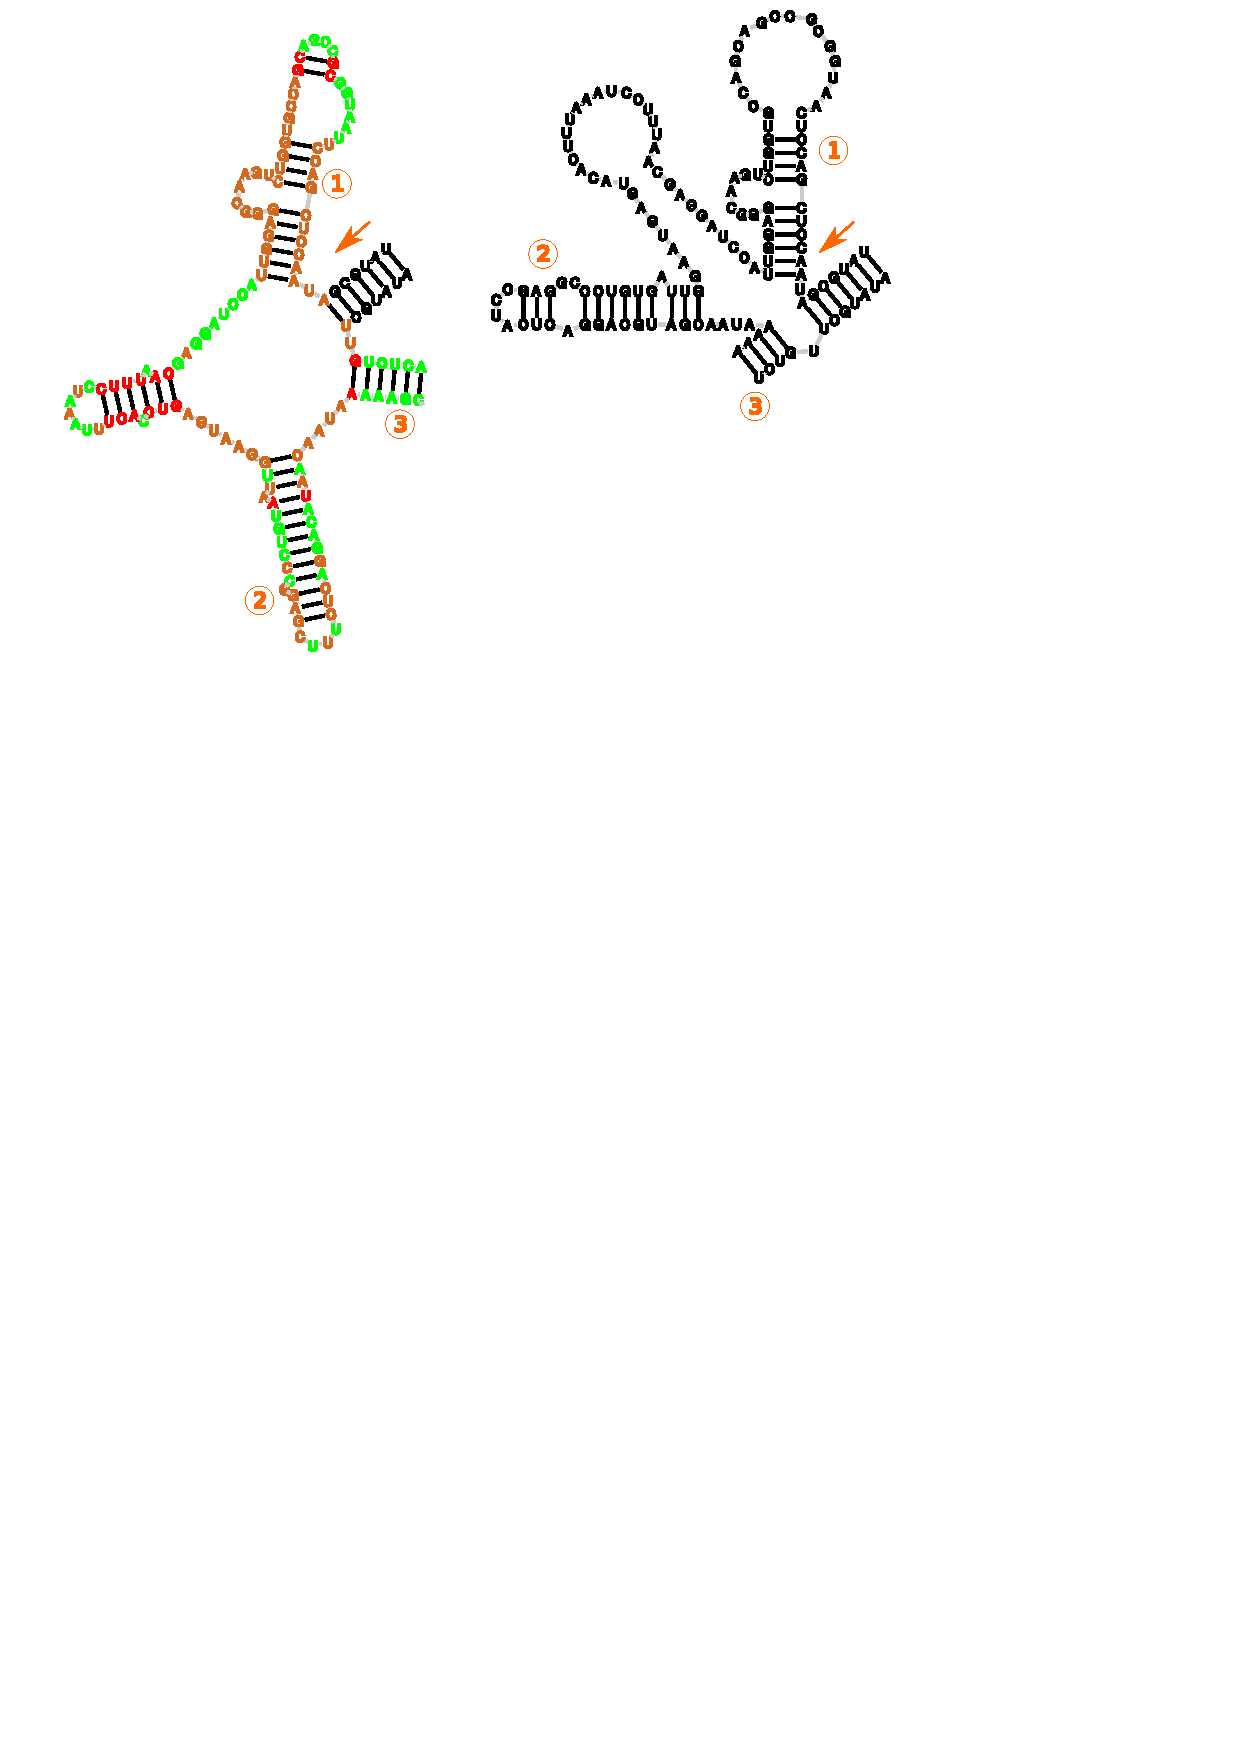
\includegraphics[clip, trim=8cm 18cm 5cm 0, width=1\textwidth]{../img/alg/insert/multibranch-redraw}
  \end{subfigure}
  \begin{subfigure}[t]{\wi}
    \caption{Kvôli vkladaniu novej vetvy sme potrebovali prekresliť celú štruktúru}
%trim=left bottom right top
    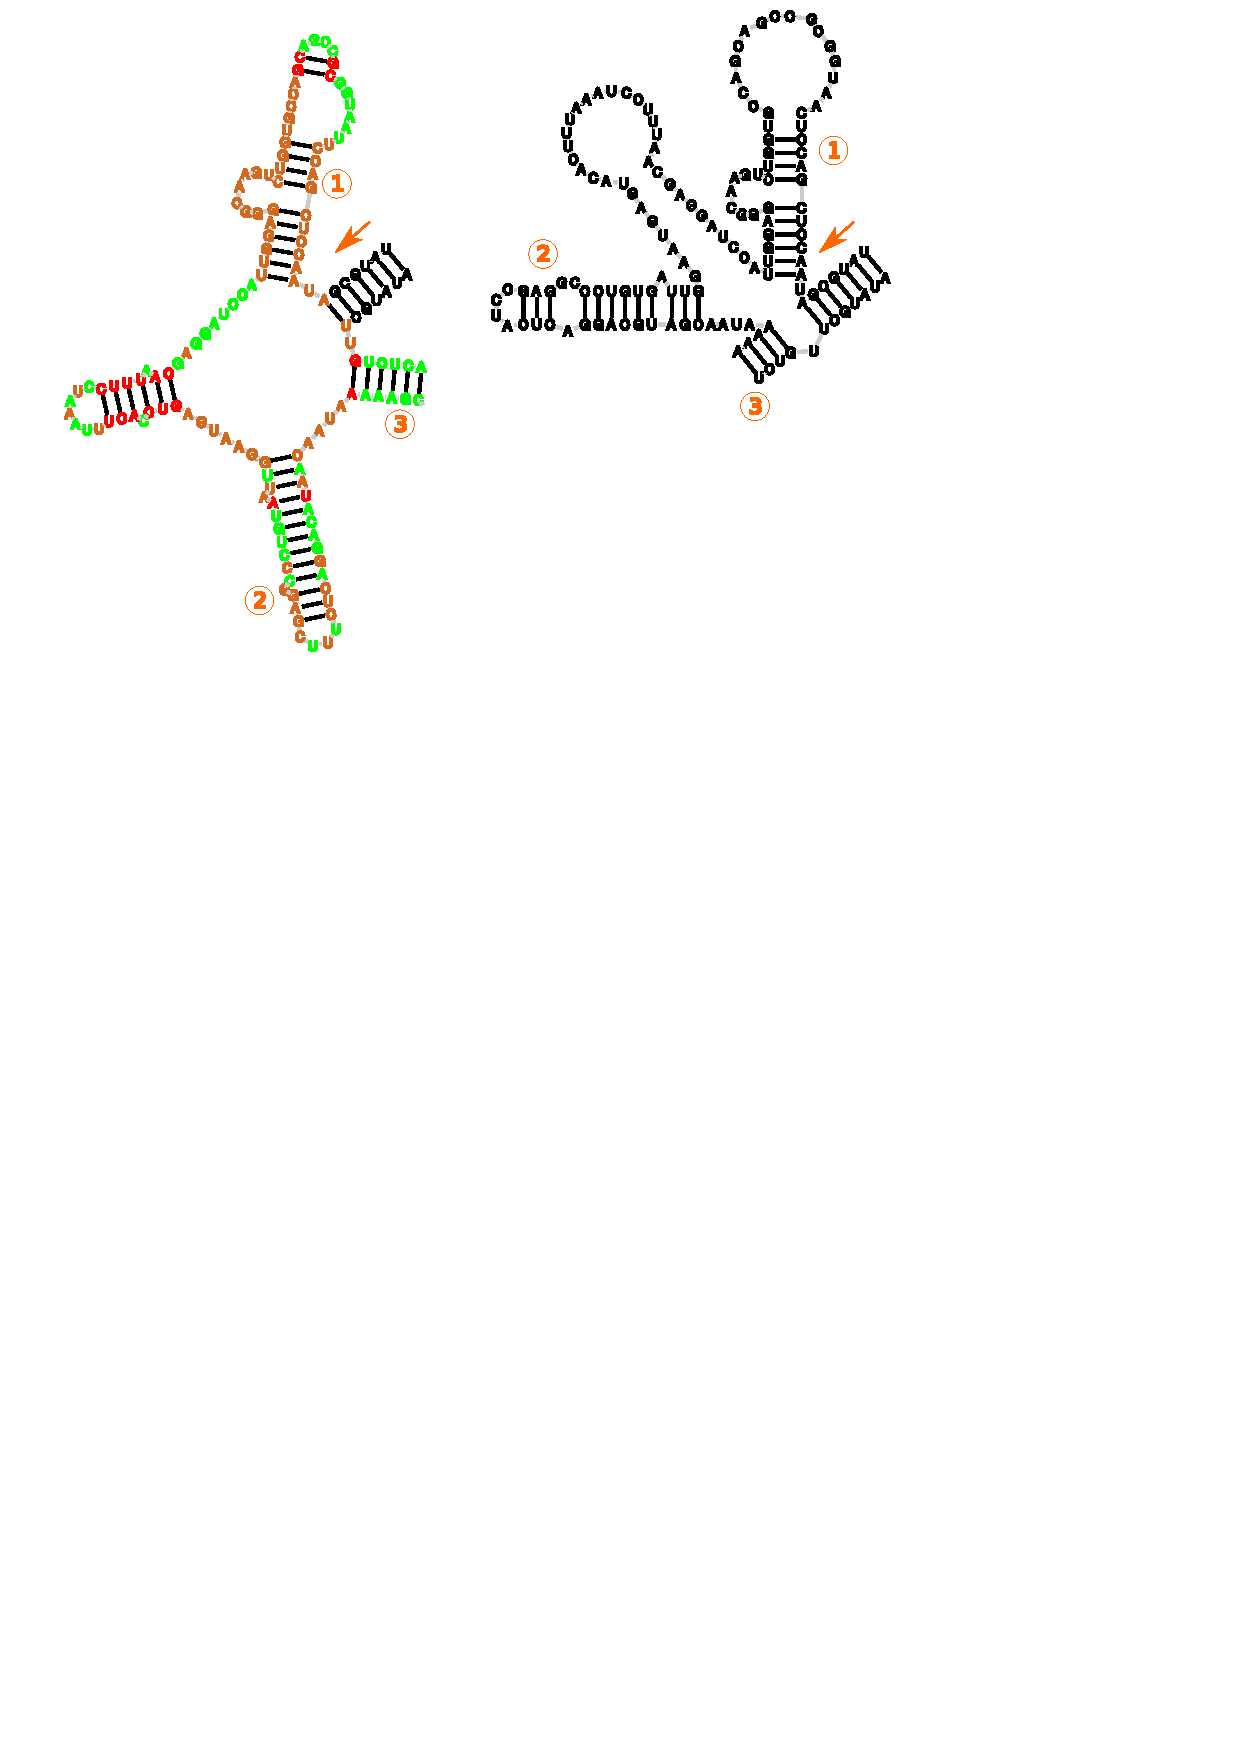
\includegraphics[clip, trim=1cm 18cm 13cm 0, width=1\textwidth]{../img/alg/insert/multibranch-redraw}
  \end{subfigure}

  \caption{Vkladanie báz do multibranch loopy s aj bez prekresľovania celej multibranch loop štruktúry}
  \label{obr:insert_multibranch}
\end{figure}





\subsection{Mazanie vrcholov zo stromu}

Mazanie považujeme za inverznú operáciu ku vkladaniu a vzhľadom k použitým operáciám
sa od neho vôbec nelíši - ak sme urobili zásah do stemu či loopu, prekreslíme
ich rovnako ako to bolo v prípade vkladania báz.




